\fancyhead[C]{Section 15.5}
	\fancyhead[R]{\dayeighteen}
	
\iftoggle{questions}{
\begin{center}{\large \textbf{Math 2551 Worksheet 18: Triple Integrals}}
\end{center}

\begin{enumerate}
	
	\item Evaluate the triple iterated integral
	\[ \int_{-1}^1\int_{0}^4\int_0^1 z^3-4x^2y\ dz\ dy\ dx. \]
	When you evaluate the innermost integral, you should treat both $x$ and $y$ as constants and take the antiderivative with respect to $z$.
	
	What is the region of integration for this integral in $\R^3$?
	
	\item Set up a triple iterated integral for $\iiint_E z\ dV$, where $E$ is the solid tetrahedron in the first octant bounded above by $x+y+z=1$. It may be helpful to make a sketch of the solid.
	
	
	\item Set up integrals that would calculate the volume of the region below, using the specified orders of integration.
	\begin{center}
		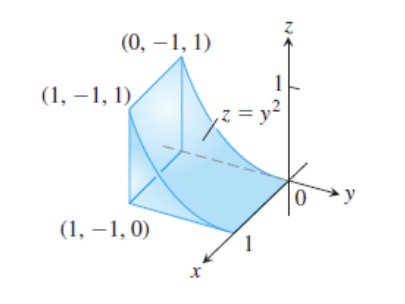
\includegraphics[scale=0.45]{15_5pic.PNG}
	\end{center}
	
	\begin{center}
		(a) $dy \ dz \ dx \quad$
		(b) $dy \ dx \ dz \quad$
		(c) $dx \ dy \ dz \quad$
		(d) $dx \ dz \ dy \quad$
		(e) $dz \ dx \ dy \quad$
	\end{center}
	
	\item Let $D$ be the region bounded by the paraboloid $z=x^2+y^2$ and the 
	plane $z=2y$, i.e. \[D=\{(x,y,z) \in \R^3 \mid x^2+y^2 \leq z \leq 2y\}.\] 
	Write triple iterated integrals in the orders $dz\ dy\ dx$ and  $dx\ dz\ dy$
	that give the volume of $D$.  Can you write a single triple iterated integral for this volume using any other orders of integration?

%%%%%%
\end{enumerate}
}{}

\iftoggle{answers}
{
	\begin{center}{\large \textbf{Math 2551 Worksheet Answers: Triple Integrals}}
	\end{center}

\begin{enumerate}
	\item $\dfrac{-58}{3}$, region of integration the rectangular prism $[-1,1]\times[0,4]\times[0,1]$ or $-1\leq x \leq 1, 0\leq y \leq 4, 0\leq z\leq 1$.

	\item Various possibilities depending on order of integration.  E.g \[\int_0^1 \int_0^{1-x} \int_0^{1-x-y}\ z\ dz\ dy\ dx \]

	\item 
	\begin{enumerate}
		\item $\displaystyle\int_0^1 \int_0^1 \int_{-1}^{-\sqrt z}\ dy \ dz \ dx $
		\item $\displaystyle\int_0^1 \int_0^1 \int_{-1}^{-\sqrt z}\ dy \ dx \ dz  $
		\item $\displaystyle\int_0^1 \int_{-1}^{-\sqrt z} \int_0^1\ dx \ dy  \ dz  $
		\item $\displaystyle\int_{-1}^0 \int_0^{y^2} \int_0^1 \ dx \ dz \ dy$
		\item $\displaystyle\int_{-1}^0  \int_0^1  \int_0^{y^2}\ dz \ dx \ dy$
	\end{enumerate}

	\item $\Ds \int_{-1}^1 \int_{1-\sqrt{1-x^2}}^{1+\sqrt{1-x^2}} \int_{x^2+y^2}^{2y} dz\ dy\ dx$.
	
		$\Ds \int_{0}^{2} \int_{y^2}^{2y} \int_{-\sqrt{z-y^2}}^{\sqrt{z-y^2}} dx\ dz\ dy$.
		
		Yes, all orders of integration result in a single iterated integral.
\end{enumerate}
}{}
\iftoggle{solutions}
{
Solutions go here in the same format.
}{}
